\documentclass{article}

\usepackage[dblblindworkshop]{neurips_2026}
\workshoptitle{AXIOM 2026} % TODO: replace with the exact official AXIOM 2026 workshop title string

\usepackage[utf8]{inputenc}
\usepackage[T1]{fontenc}
\usepackage{hyperref}
\usepackage{url}
\usepackage{booktabs}
\usepackage{amsfonts}
\usepackage{amsmath}
\usepackage{nicefrac}
\usepackage{microtype}
\usepackage{xcolor}
\usepackage{graphicx}

\title{Raw Hessian Trace Better Identifies Quantization-Damaged Layers Than the HAWQ Product Under Power-of-Two Quantization}

\author{%
  Anonymous Author(s) \\
  Affiliation \\
  Address \\
  \texttt{email} \\
}

\begin{document}

\maketitle

\begin{abstract}
Hessian-based curvature analyses (the HAWQ family) are an established tool for quantization-sensitivity ranking, typically combining curvature and perturbation magnitude into a single product, $\mathrm{Tr}(H)\cdot\|\Delta W\|^2$, to guide mixed-precision assignment. We test this formulation directly against measured per-layer weight-quantization damage under Power-of-Two (PoT) encoding, across three CNN architectures (a compact CNN, ResNet-18, ResNet-50) on two datasets (ImageNet100, CIFAR10; post-training quantization). Raw curvature $\mathrm{Tr}(H)$ identifies the true single most-damaged layer at rank~1 in 3 of 6 architecture$\times$dataset combinations, and its overlap with the five truly most-damaged layers is never worse than the HAWQ-V2 product's or the perturbation term's, which never win outright. Which specific layer is most damaged is itself dataset-dependent: the network's stem convolution dominates on ImageNet100, but not always on CIFAR10, where damage can be small and diffuse (ResNet-50: 1.6 accuracy points total, no predictor performs well). Full-ranking Spearman correlation is weak and mostly non-significant throughout; robust top-$k$ identification, not full-distribution correlation, is the finding that survives across datasets.
\end{abstract}

\section{Introduction}

Efficient inference on resource-constrained hardware makes weight quantization a central problem in deploying neural networks. Power-of-Two (PoT) quantization is a particularly hardware-attractive scheme: because PoT weights are exact powers of two, multiply-accumulate operations reduce to bitshifts, avoiding multipliers entirely \citep{miyashita_pot_2016,przewlocka_rus_pot_2022}. This efficiency is not free: post-training PoT quantization (PTQ) costs 8.8--18.0 accuracy points on ImageNet100 and 1.4--10.2 points on CIFAR10, depending on architecture, with substantial variation in \emph{which} layers absorb this damage.

The HAWQ family addresses this by using curvature as a sensitivity signal for mixed-precision decisions. HAWQ \citep{dong_hawq_2019} ranks layers by the top Hessian eigenvalue; HAWQ-V2 \citep{dong_hawqv2_2020} refines this into a curvature-times-perturbation product, $\mathrm{Tr}(H)\cdot\|\Delta W\|^2$, motivated by a second-order Taylor expansion of the loss. Per-layer traces are estimated efficiently via Hutchinson's method, as implemented in PyHessian \citep{yao_pyhessian_2020}.

HAWQ uses this formulation to \emph{decide} bit-width allocation, but the underlying predictive claim, that $\mathrm{Tr}(H)\cdot\|\Delta W\|^2$ tracks actual per-layer damage, is rarely tested directly against measured damage. This is particularly relevant under PoT: unlike uniform quantization, PoT's non-uniform grid means a layer's perturbation size depends on how well its weight distribution happens to align with grid points, not primarily on layer size or precision, so the predictive power of the HAWQ-V2 product under PoT is untested.

We test three predictors, raw curvature $S_{raw}=\mathrm{Tr}(H)$, perturbation magnitude $S_{pert}=\|\Delta W\|^2$, and the HAWQ-V2 product $S_{hawq}=\mathrm{Tr}(H)\cdot\|\Delta W\|^2$, against measured per-layer weight-quantization damage on three CNN architectures and two datasets (six combinations total). We show: (1) raw curvature identifies the true top-damage layer at rank~1 in half of the six combinations, and never has worse top-5 overlap with true damage than the other two predictors, which never win outright; (2) which layer is most damaged, and how well any predictor finds it, depends on the dataset and on how concentrated total damage is, diffuse low-damage regimes (ResNet-50/CIFAR10) defeat all three predictors; (3) careful canonical trace measurement matters: we document a previously unresolved two-order-of-magnitude discrepancy between historical and canonical trace values for the same nominal quantity in our own pipeline.

Our analysis is scoped to weight quantization. Under PTQ, isolated weight-only damage matches or exceeds total joint damage in every architecture on both datasets we test, while isolated activation-only damage is negligible (within $\pm0.4$ points, sometimes slightly negative) in every case. This motivates weight damage as the practically dominant and cleanly definable isolation target here. Activation quantization is known to follow a different, outlier-driven failure mode \citep{xiao_smoothquant_2023,lin_awq_2024}, and we do not address it.

\section{Related Work}

\textbf{Hessian-based quantization sensitivity.} HAWQ \citep{dong_hawq_2019} uses the top Hessian eigenvalue to guide mixed-precision bit-width assignment; HAWQ-V2 \citep{dong_hawqv2_2020} refines this to a curvature-times-perturbation sensitivity product motivated by a second-order Taylor expansion of the loss. Both use per-layer Hessian trace estimates obtained via Hutchinson's stochastic estimator, popularized as a standard toolkit by PyHessian \citep{yao_pyhessian_2020}, which we also use here.

\textbf{Structure of the Hessian spectrum.} \citet{sagun_singularity_2016} and \citet{sagun_empirical_2017} document a bulk-plus-outlier structure in trained networks' Hessian spectra, consistent with a random-matrix-theory picture in which most eigenvalues cluster near zero while a small number of large outliers dominate. \citet{karakida_fisher_2019} derive mean-field predictions for the Fisher/Hessian spectrum at random initialization. Our finding that a single layer's curvature often dominates its network, though not always the same layer or with the same margin across datasets, is consistent with this outlier picture without directly testing its random-matrix-theory predictions.

\textbf{PoT quantization and activation outliers.} PoT was proposed as a hardware-friendly logarithmic weight representation \citep{miyashita_pot_2016}, with its bitshift-based efficiency motivated further for low-bitwidth hardware compliance \citep{przewlocka_rus_pot_2022}. On the activation side, which we exclude from our scope, SmoothQuant \citep{xiao_smoothquant_2023} and AWQ \citep{lin_awq_2024} establish that activation quantization fails through systematic, channel-wise outliers rather than curvature; BRECQ \citep{li_brecq_2021} addresses post-training quantization more broadly via block-wise reconstruction.

\section{Methods}

\subsection{Trace measurement}
We estimate per-layer Hessian trace with PyHessian's Hutchinson estimator \citep{yao_pyhessian_2020} using Rademacher probes. To keep results reproducible under configuration choices that the literature usually leaves implicit, we fix a canonical configuration: mean-reduced cross-entropy loss, a fixed validation batch, three probe seeds (42, 43, 44) averaged into a mean$\pm$std per layer, deterministic algorithms, and \texttt{eval()} mode. Probe budget is matched within each dataset but differs across them (CIFAR10: 80 images, 100 Hutchinson iterations; ImageNet100: 24 images, 30 iterations, reduced because per-iteration Hessian-vector-product cost is far higher at $224\times224$ than at $32\times32$). We report the fused-BatchNorm basis as canonical for cross-stage comparison, since PTQ and QAT checkpoints exist only in fused form; FP32 models are traced in both unfused and fused bases so the fusion effect is never hidden. Because PTQ/QAT weights are quantized with a straight-through estimator, the Hessian evaluated on these models is the STE-relaxed loss curvature \citep{bengio_ste_2013}, not the classical Hessian of an unquantized network.

\subsection{Weight-only damage isolation}
For each layer $l$ we define $\mathrm{weight\_damage}(l) = \mathrm{acc}_{fp32} - \mathrm{acc}_{iso}(l)$, where $\mathrm{acc}_{iso}(l)$ is the accuracy of a model in which \emph{only} layer $l$'s weights are PoT-quantized; all other weights and all activations remain FP32. Because isolated single-layer quantization can slightly \emph{improve} accuracy for some layers, we use $\mathrm{abs\_weight\_damage}(l) = |\mathrm{weight\_damage}(l)|$ as the target for predictor comparison.

\subsection{Three predictors}
We compare three per-layer sensitivity scores against $\mathrm{abs\_weight\_damage}(l)$: raw curvature $S_{raw}(l) = \mathrm{Tr}(H_l)$ (canonical fused basis, evaluated on the FP32 model, as in HAWQ-style usage); perturbation magnitude $S_{pert}(l) = \|W_l - Q(W_l)\|^2$; and the HAWQ-V2 product $S_{hawq}(l) = \mathrm{Tr}(H_l)\cdot\|W_l - Q(W_l)\|^2$ \citep{dong_hawqv2_2020}. We evaluate each via Spearman rank correlation, the rank each predictor assigns to the layer of true maximum damage, and overlap between each predictor's top-5 and the true top-5 damaged layers.

\section{Results}

\subsection{Setup}
We study three architectures, a compact CNN (6 quantizable layers), ResNet-18 (21 layers), and ResNet-50 (54 layers), on two datasets (CIFAR10, ImageNet100), quantized post-training (PTQ) with PoT weight encoding, six architecture$\times$dataset combinations in total. All numbers below are for PTQ.

\subsection{Which layer is most damaged is dataset-dependent}
In every combination, one layer absorbs disproportionately more weight-quantization damage than the rest (Figure~\ref{fig:main}), but which layer this is depends on the dataset. On ImageNet100 it is always the stem convolution \texttt{conv1} (3.72, 5.34, 7.30 points for ResNet-18/-50/CNN, out of 8.8--18.0 total). On CIFAR10 it is \texttt{conv1} only for the CNN (5.63 of 10.2 total points); for the ResNets a different layer takes over, \texttt{layer1.1.conv1} for ResNet-18 (0.78 of 1.4 total points) and the final fully-connected layer for ResNet-50 (0.57 of only 1.6 total points), reflecting CIFAR10's far smaller and more diffusely spread PTQ damage.

\begin{table}[t]
\centering
\caption{Rank assigned by each predictor to the true top-damage layer (1 = best), and each predictor's overlap with the true top-5 damaged layers (out of 5), per architecture$\times$dataset combination, PTQ.}
\label{tab:rank}
\small
\begin{tabular}{llccccc}
\toprule
Dataset & Model ($n$) & top-damage layer & $S_{raw}$ rank & $S_{raw}$ top5 & $S_{pert}$ top5 & $S_{hawq}$ top5 \\
\midrule
ImageNet100 & CNN (6)        & \texttt{conv1}         & 3  & 4/5 & 4/5 & 4/5 \\
ImageNet100 & ResNet-18 (21) & \texttt{conv1}         & \textbf{1} & 1/5 & 1/5 & 1/5 \\
ImageNet100 & ResNet-50 (54) & \texttt{conv1}         & \textbf{1} & 1/5 & 0/5 & 0/5 \\
CIFAR10     & CNN (6)        & \texttt{conv1}         & 2  & 5/5 & 4/5 & 5/5 \\
CIFAR10     & ResNet-18 (21) & \texttt{layer1.1.conv1}& \textbf{1} & 2/5 & 0/5 & 0/5 \\
CIFAR10     & ResNet-50 (54) & \texttt{fc}            & 40 & 1/5 & 0/5 & 0/5 \\
\bottomrule
\end{tabular}
\end{table}

Table~\ref{tab:rank} summarizes how well each predictor identifies this layer. $S_{raw}$ achieves exact rank-1 identification in 3 of 6 combinations, and its top-5 overlap is never worse than $S_{pert}$'s or $S_{hawq}$'s in any combination, strictly better in half. $S_{pert}$ never achieves rank-1 identification, and buries the true top-damage layer near the bottom of the ranking whenever that layer is a low-fan-in convolution (\texttt{conv1}, \texttt{layer1.1.conv1}; see Figure~\ref{fig:main}). $S_{hawq}$, inheriting $S_{pert}$'s perturbation term, likewise never achieves rank-1 identification and never exceeds $S_{raw}$'s top-5 overlap. The one combination where all three predictors fail, ResNet-50/CIFAR10, is also the combination with the smallest, most diffuse total damage (1.6 points across 54 layers); we take this as evidence that a usable curvature signal requires damage concentrated enough to separate from noise, not a failure specific to any one predictor.

\begin{figure}[t]
\centering
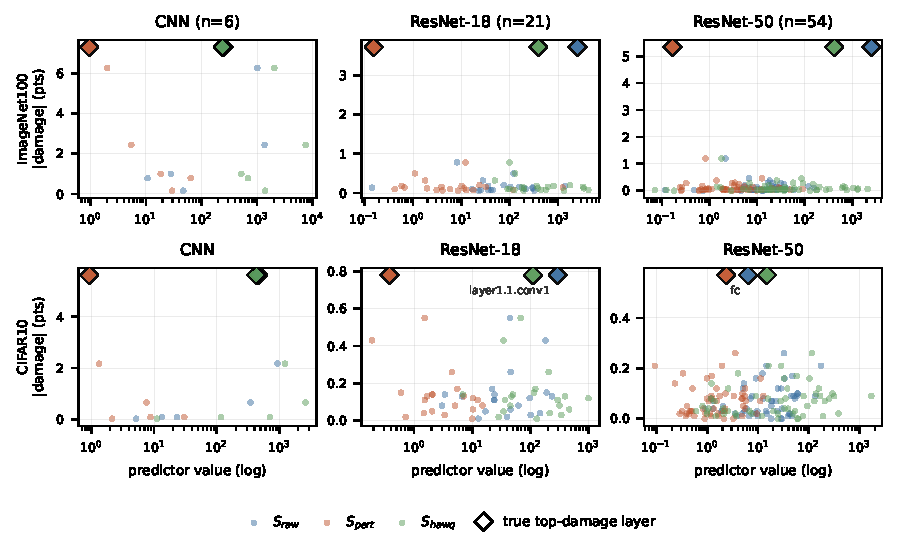
\includegraphics[width=\linewidth]{figures/main_figure.pdf}
\caption{Per-layer predictor value (log scale) vs.\ measured $|\mathrm{weight\_damage}|$, PTQ; top row ImageNet100, bottom row CIFAR10. Diamonds mark each architecture's true top-damage layer (labeled where not \texttt{conv1}). $S_{raw}$ (blue) tracks it well in 4 of 6 panels; $S_{pert}$ (orange) never does.}
\label{fig:main}
\end{figure}

\subsection{Full-ranking correlation is weak}

\begin{table}[t]
\centering
\caption{Spearman rank correlation ($\rho$, $p$-value) between each predictor and $\mathrm{abs\_weight\_damage}$, PTQ, all layers per combination. Bold: $p<0.05$.}
\label{tab:corr}
\small
\begin{tabular}{llccc}
\toprule
Dataset & Model ($n$) & $S_{raw}$ & $S_{pert}$ & $S_{hawq}$ \\
\midrule
ImageNet100 & CNN (6)        & 0.60 (0.21)          & \textbf{$-0.94$ (0.005)} & $-0.14$ (0.79) \\
ImageNet100 & ResNet-18 (21) & 0.12 (0.60)           & $-0.25$ (0.27)           & $-0.15$ (0.51) \\
ImageNet100 & ResNet-50 (54) & \textbf{0.30 (0.028)} & $-0.01$ (0.96)           & 0.18 (0.20) \\
CIFAR10     & CNN (6)        & \textbf{0.93 (0.008)} & $-0.64$ (0.17)           & 0.55 (0.26) \\
CIFAR10     & ResNet-18 (21) & 0.29 (0.20)            & $-0.36$ (0.11)           & $-0.16$ (0.49) \\
CIFAR10     & ResNet-50 (54) & 0.21 (0.14)            & 0.18 (0.20)              & 0.19 (0.16) \\
\bottomrule
\end{tabular}
\end{table}

Table~\ref{tab:corr} shows only 3 of 18 (predictor$\times$architecture$\times$dataset) correlations reach $p<0.05$: $S_{raw}$ for CNN on both datasets and for ResNet-50/ImageNet100, and $S_{pert}$ for CNN/ImageNet100. No $S_{hawq}$ correlation reaches significance on either dataset, and $S_{pert}$'s sign is not even consistent across datasets (weakly positive for ResNet-50/CIFAR10, essentially zero for ResNet-50/ImageNet100, strongly negative for CNN). Given heavy-tailed and often diffuse damage distributions, we treat top-$k$ identification (Table~\ref{tab:rank}), not full-distribution correlation, as the more robust cross-dataset summary.

The dataset-dependence in \S4.2 has a plausible architectural reading: CIFAR10's lower input resolution and correspondingly milder overall PTQ damage leave less headroom for any single layer to dominate, so the network's largest curvature outlier (\texttt{conv1}, 2.5--11.7$\times$ its model's median layer trace on CIFAR10 vs.\ 34--150$\times$ on ImageNet100) does not always coincide with the largest damage outlier. This changes \emph{whether} a clear outlier exists to find, not which predictor performs best when one does.

\section{Discussion and Limitations}

HAWQ-V2's product is motivated by a second-order Taylor expansion, $\Delta L \approx \frac{1}{2}\Delta W^\top H \Delta W$, which implicitly assumes $\|\Delta W\|^2$ is comparable in scale across layers, so that curvature dominates the ranking. This is a reasonable approximation under uniform quantization, where perturbation size scales predictably with a layer's bit-width and weight range. Under PoT it breaks down: perturbation size depends on how well a layer's specific weight values happen to align with the PoT grid, which is close to incidental for a small, low-fan-in stem-like kernel. More precisely, the product only behaves as ``sensitivity'' if $\|\Delta W\|^2$ is at least uncorrelated with a layer's curvature-based sensitivity; PoT structurally violates this, since grid alignment is a property of a layer's weight distribution, independent of its curvature, and for \texttt{conv1} the two are directly opposed (highest sensitivity, smallest perturbation). This is why an established, widely used sensitivity formulation misleads specifically under this quantization scheme, not a general failure of curvature-based sensitivity, and it holds regardless of which layer happens to be most damaged in a given architecture or dataset.

As a methodological aid, not a novel contribution in itself: canonical trace measurement matters more than the literature typically documents. In our own pipeline, two historical, differently-configured runs produced ResNet-50 \texttt{conv1} PTQ trace values of 13161.8 and 1030.9, against our canonical re-measurement of 97.8, a gap of two orders of magnitude for the nominally same quantity that a systematic sweep over basis, loss reduction, probe count, and data source could not reconcile with either historical value. We report a fixed canonical configuration and both fused/unfused bases explicitly throughout so our own predictor comparison is at least internally reproducible, and recommend the same discipline for future curvature-based quantization-sensitivity work.

\textbf{Limitations.} (1) One training run per architecture per dataset; cross-seed variance in the top-damage-layer finding is not characterized. (2) Probe budgets differ between datasets (\S3.1) and are not matched, so trace-estimation noise could itself contribute to CIFAR10's weaker correlations, independent of any genuine dataset effect. (3) We analyze PTQ only; QAT per-layer sensitivity, where isolated damage can also be negative, is left to future work. (4) A naive Kronecker-factored (KFAC-style) approximation \citep{martens_kfac_2015,grosse_kfc_2016} underpredicts the measured per-parameter trace at every architecture's top-damage-adjacent layers by many orders of magnitude (network-wide median $\approx$5.5--6.2, vs.\ 7.1--9.8 at \texttt{conv1} specifically) on both datasets, so it does not explain these layers' curvature; the architectural cause remains open. (5) Our findings are specific to PoT quantization; applicability to uniform int8 or mixed-precision schemes is untested.

\section{Conclusion}
Raw canonical Hessian trace identifies the true top-damage layer at rank~1 in half of the six architecture$\times$dataset combinations we test, and never has worse top-5 overlap with true weight-quantization damage than the HAWQ-V2 product or the perturbation term alone, across three CNN architectures on both ImageNet100 and CIFAR10 under PoT quantization. Which specific layer is most damaged is itself dataset-dependent, and where total damage is small and diffuse (ResNet-50/CIFAR10), no predictor we test performs well. Curvature-based sensitivity formulations therefore need quantization-scheme- and damage-regime-specific adaptation rather than a single universal product. Future work includes a random-matrix-theory-informed decomposition of the bulk-versus-outlier spectrum, matching probe budgets across datasets to isolate estimation noise from genuine dataset effects, and systematic extension to uniform and mixed-precision quantization schemes.

\bibliographystyle{plainnat}
\bibliography{reference}

\end{document}
